%preamble
\documentclass[12pt,a4paper]{article}

%inputs for firstpage
\def \CourseName {گزارش فاز سوم}
\def \Instructor {دکتر مسلم حبیبی}
\def \Semester {نیم‌سال دوم\\سال تحصیلی 99-00}


%packages
\usepackage[]{algorithm2e}
\usepackage{cite}
\usepackage{calc}
\usepackage{fancyhdr}
\usepackage{lipsum}
\usepackage{color}
\usepackage{ragged2e}
\usepackage[inline]{enumitem}
\usepackage[dvipsnames]{xcolor}
\usepackage{graphicx}
\usepackage{wrapfig}
\usepackage{float}
\usepackage[skip=12pt,indent=2em]{parskip}
\usepackage{setspace}
\usepackage{textcomp}
\usepackage{etoolbox}
\usepackage{xpatch}
\usepackage{tabu}
\usepackage{hyperref}


%for persian fonts
\usepackage{xepersian}
\defpersianfont\bnazanin{BNazanin}
\settextfont{BNazanin}

\title{
	\center
	
\includegraphics[width=5cm, height=5cm]{images/shariflogo.jpg} \\
	دانشکده مهندسی صنایع \\
	دانشگاه صنعتی شریف \\
	\CourseName
}
\author{
	\\
	\\
	\textbf{استاد درس:}
	\\
	\Instructor \\[35pt]
	\\
	\textbf{نام اعضای گروه:}
	\\مهدی محسنی 
	\\محراب کشاورز گیلده 
	\\احسان چشمی
	\\[45pt]
}
\date{{\small\Semester}}



%body
\begin{document}

\maketitle
\pagebreak
\tableofcontents
\pagebreak
\listoffigures
\pagebreak
\normalsize	



\pagebreak
\section{رسم فرایندها} \label{section.function}

\subsection{فرایند ثبت نام} \label{section.function.register}


\subsection{فرایند خرید} \label{section.function.buy}


\subsection{فرایند مرجوعی} \label{section.function.return}

در ابتدا مشتری وارد حساب کاربری خودش می شود. لیست خریدی که داشته را انتخاب می کند. کالایی را که می خواهد مرجوع بزند انتخاب می کند. مشخصات کالا، دلایل پس دادن آن و اطلاعات زمانی و مکانی پس دادن کالا را مشخص می کند. در صورت عدم موافقت با درخواست و نداشتن شرایط لازم برای پس دادن کالا درخواست رد می شود. در صورت موافقت سامانه به دنبال نزدیک ترین پیک می رود و همچنین اطلاعات کالای مرجوعی را به صاحب فروشگاهی که محصول را فروخته بود می دهد. نزدیک ترین پیک که پیدا شد مشخصات کالای مرجوعی برای او ارسال می شود در صورت عدم موافقت او سامانه به دنبال نزدیک ترین پیک بعدی می رود. در صورت موافقت پیک به مکان مورد نظر مشتری در زمان تعیین شده از قبل می رود تا کالای مرجوعی را تحویل گیرد. فروشگاه مبلغ کالای مرجوعی را برای حساب سامانه واریز می کند. سامانه پول دریافتی را برای حساب مشتری واریز می کند. پس از اتمام واریز پول و رفتن پیک و تحویل کالای مرجوعی آن کالای مرجوعی به فروشگاه برگردانده می شود.

\section{گزارش نحوه انجام پروژه} \label{section.report}

\subsection{جلسه \lr{post mortem}} \label{section.report.postMortem}
این مطلب مربوط به اسپرینت چهارم است.

\subsection{\lr{Task board and Burndown Chart}} \label{section.report.taskBoard}

	\begin{figure}[h!]
	\begin{center}
		\includegraphics[width=14cm]{images/screenshot_7.png}	
	\end{center}
	\caption{ابتدای اسپرینت}
\end{figure}

\begin{figure}[h!]
	\begin{center}
		\includegraphics[width=14cm]{images/screenshot_1.png}
	\end{center}
	\caption{انتهای اسپرینت}
\end{figure}


%\begin{figure}[h!]
%	\begin{center}
%		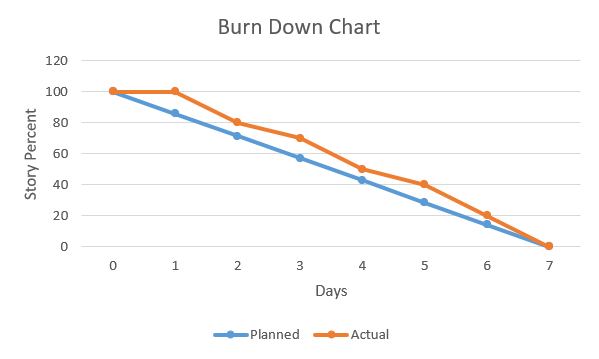
\includegraphics[width=14cm]{images/Burn Down Chart.png}
		
%	\end{center}
%	\caption{\lr{Burn Down Chart}}
%\end{figure}




\end{document}